%!TEX root = ../thesis.tex
\chapter{Influence Detection \& Ranking Stability }\label{ch:ranking}

% \epigraph{Simplicity is a great virtue but it requires hard work to achieve it and education to appreciate it. And to make matters worse: complexity sells better.}{Edsger Wybe Dijkstra}

\epigraph{Everything should be made as simple as possible, but not simpler.}{Albert Einstein, {\em commonly paraphrased quote from his Herbert Spencer Lecture}, Oxford, June 10, 1933.}

Complex networks are powerful tools to encapsulate and probe deeper aspects of systems; however, this can often come at the cost of human interpretability. Answering questions is a important task for such networks, but simplifying networks to answer questions can be fraught with challenges.

In this chapter we will examine the use of the network created in \autoref{ch:quotermodel} to explore the process of answering a specific question: which news-media organisations are the most important information sources? In essence, this question is one of ranking the news-media organisations according to their importance to the information flow network. 

While ranking is often assumed to be a simple task, we will show in this chapter that different approaches to ranking a influence network can result in vastly different answers. Such approaches are built upon assumptions of importance that are often inconsistent with one another. Even standalone these approaches can exhibit unexpected sensitivities to changes in the network.

This chapter will not produce a definitive ranking of importance, but rather will use the question to explore the difficulty in constructing such an answer from a complex network. Doing so reveals the interconnected nature of the information flow ecosystem and its resistance to simplification.

% We will show that there are many approaches to achieve this, each with their own justifications and shortcomings. Such approaches - even when well formulated - can have unexpected sensitivities to changes in the network and ranking consensus across methods is rare. Extreme care should be taken when attempting to answer such a question from a network, especially in contexts where small decisions can have significant impacts on results.


\section{Spotify: A motivating example}

Recent work by South \emph{et al.}~\cite{south_centrality_2021} has looked into the stability of eigenvector centrality in the network of musical artist collaborations using data from Spotify. This work collected the discography, genre, popularity and other metadata for over 1.25 million artists using the online music streaming platform. From the discography, a network of artists was created with edges indicating that two artists appear on an piece of music together. 

Such a collaboration network leads to a natural question; who are the most important musical artists? Eigenvector centrality (discussed further below) is applied to this large undirected network to create a ranking of how important an artist is the full network. In this calculation the popular classical artists are ranked highest in centrality. The most popular artist being Mozart followed closely by Bach, Beethoven and Schubert. This result, interesting in its own right, is not what troubles us.

Popularity in Spotify is a value between 0 and 100 based on relative music streams, which is a strongly skewed distribution resulting in a large number of low popularity artists. An experiment was run where artists with a popularity less than some threshold number were removed from the network.  Such a hypothetical situation is not uncommon in practice, where challenges in data collection or limits of computation on large graphs can naturally lead to decisions to discard data below certain thresholds of relevancy.

When centralities are re-calculated on networks with artists below a popularity threshold removed, the results change. For thresholds between 1 and 46, small perturbations in the rankings occur but general trends persist. However, at a threshold of 47 the centrality rankings change {\em en masse} to a central core of popular rap artists (Rick Ross, Lil Wayne, T.I and others). These new rankings remain consistent as thresholding increases.

This critical transition in centrality is shown in \autoref{fig:rank_spotify_shift_a}. The transition is not caused by the removal of any key artists in the graph but rather by a swapping of dominant and secondary eigenvectors as shown in \autoref{fig:rank_spotify_shift_b}. This is further validated using a novel network model by the authors and has been observed in the context of the HITS centrality~\cite{ng_link_2001}.


\begin{figure}[!htbp]
	\centering
	\begin{subfigure}[t]{\textwidth}
		\centering
		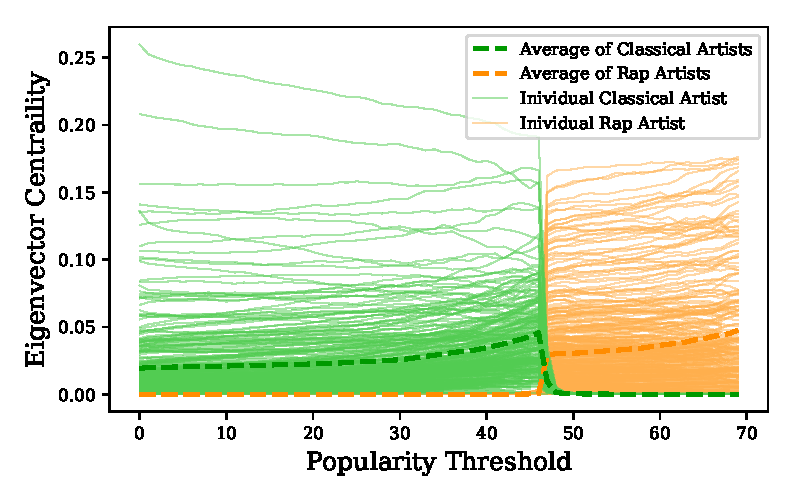
\includegraphics[width=0.7\textwidth]{chapter4/figs/spotify_a.pdf}
		\caption{Changing Centralities}
		\label{fig:rank_spotify_shift_a}
	\end{subfigure}
	~
	\begin{subfigure}[t]{\textwidth}
		\centering
		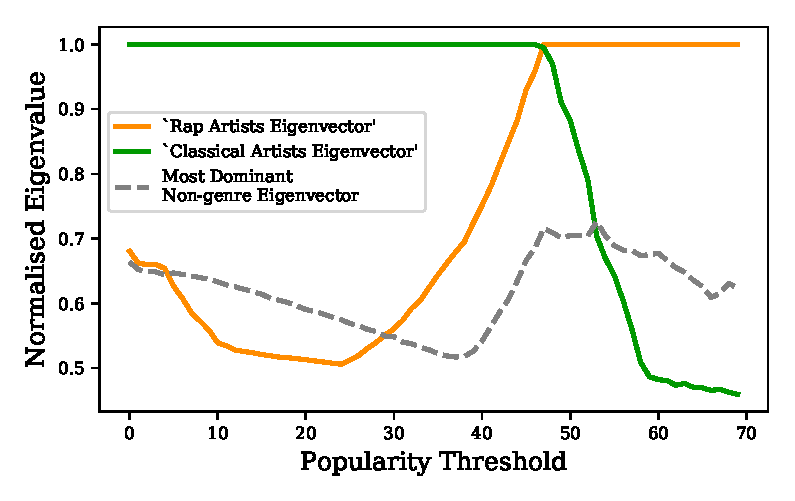
\includegraphics[width=0.7\textwidth]{chapter4/figs/spotify_b.pdf}
		\caption{Changing Eigenvalues}
		\label{fig:rank_spotify_shift_b}
	\end{subfigure}
	\caption{Change in centrality of all classical artists and all rap artists in the Spotify artist collaboration graph as a popularity threshold is applied. Artists of other genres have negligible centrality. In (a), the critical transition in centrality between the two groups can be seen at a threshold of 46. In (b) the changes in the most dominant eigenvalues of the adjacency matrix are shown as popularity thresholding is applied to the network. Eigenvalues are normalised to the largest eigenvalue and are labelled according the group of nodes with high centrality in the corresponding eigenvectors. A swap between the dominant eigenvectors can be seen, corresponding to the critical transition in centrality.}
\end{figure}

The purpose of this example is to highlight a key issue. Centralities and rankings can be susceptible to critical changes even from small perturbations in the data. This certainly does not make for a good ranking, but how does one measure a `good' ranking?


\section{Rank Stability}

There are many criteria with which one can judge a ranking system: a notion of `truthfulness'; a desire for resistance to being `gamed'; or a desire for consistency of the ranking when small changes occur. Though not an exhaustive list, these are fair criteria, but are rife with issues. So let's use these building blocks to construct some more robust metrics.

Every ranking method is truthful to it's own definition, but generalising this to a Platonic ideal is difficult. Instead we could seek a unanimity between rankings. As we will see below, there are usually a large number of possible ranking approaches to any given problem. A good set of ranking methods should produce similar rankings when drawing upon similar definitions and assumptions.

Creating resistance to undue manipulation is a difficult problem, not only because defining `undue' is problematic. Any system of ranking must be manipulated by the results of comparisons between elements. The issues arise when a single element, player, or node can alter the rankings dramatically though only it's behaviour. In our context of ranking news information influence we will use a simple definition. We want to minimise the influence that a single addition of removal of a node from the network has on the rankings.

This definition sits close to our third criterion, consistency of ranking. When a small change in the graph occurs, such as the removal of a single node, we would want the ranking change to be correspondingly small. This desire for rank stability stands in contrast to the motivating example above, where the centrality ranking underwent a total overhaul during a critical transition. This is something a strong ranking should avoid. Further to this, consistency of ranking should be maintained across rankings, especially when these ranking methods are similar in nature. 


\subsection{Ranking Methods}

Before diving deeper into this discussion, lets first define some methods of ranking the news-media outlets in our network. A vast array of ranking methods exist, but not all are suited to any one problem. In our problem, we want to rank influence in a weighted directed network. Here we will use four methods for comparison: two network centralities, a method of sport team ranking, and a network topology approach. We will also outline why many alternative metrics are not useful in this context. This list of methods is not exhaustive, but provides a substantive example of several approaches which will allow for an analysis of the viability of ranking influence in an information flow network. 

\subsubsection{Network Centralities}

Network centrality metrics are a common tool for measuring different notions of importance within a network. However, these notions of importance are often context specific. For example, betweenness centrality is a powerful metric that measures the number of shortest paths that pass through a node. This centrality is very useful in a context such a packet routing and load balancing, where a comparatively high value in the centrality (and thus a low rank) would indicate a high burden of traffic and the importance of reliability of that node. In the context of our question, this centrality doesn't illuminate who \emph{contributes} the information, but rather what nodes have the most \emph{pass-through} of information. In a similar vein, centralities such as degree and closeness also provide answers to questions we are not asking here.

A centrality measure that has the characteristics we are looking for is \emph{eigenvector centrality}. Eigenvector centrality, sometimes referred to as \emph{eigencentrality}, is defined recursively in terms of the centrality of a node's neighbourhood. This stems from the notion that a node is important if it is connected to other important nodes. In our context of information flow we can restate this as: a node is an important contributor of information if it contributes to other important information contributors. In essence, if a node contributes to a few unimportant nodes, it itself is unimportant; but those nodes that contribute to influential sources, are themselves influential.

This importance rating is encapsulated in a vector $v^{\rm(eig)}$ which is defined through the recursive equation
\begin{equation}\label{eq:eigenvector}
\textbf{v}_{i}^{\rm(eig)}=\frac{1}{\lambda} \sum_{k=1}^{N} A_{k, i} \textbf{v}_{k}^{\rm(eig)},
\end{equation}
with a constant $\lambda \neq 0$ and where $A_{k, i}$ is the element of the weighted adjacent matrix of the graph, $A$, with $N$ total nodes. This can then be expressed in matrix form as,
\begin{equation}
\lambda v^{\rm(eig)} = A v^{\rm(eig)}, 
\end{equation}
which can be solved as the dominant left-hand eigenvector of the adjacency matrix $A$. 

Importantly, both here and below, the direction of `flow' in the graph (the direction of each edge) is reversed before taking this calculation. Eigenvector centrality works such that the node \emph{being pointed to} is assigned the importance. Since we are interested in what originates information, we must point \emph{towards} the information source.

Eigenvector centrality has been shown to be more robust to conditions of imperfect data~\cite{costenbader_stability_2003} and network manipulation \cite{niu_robustness_2015} than other centrality measures, but can undergo critical transitions when the eigengap is very small~\cite{south_centrality_2021}.

Similar to eigenvector centrality, \emph{PageRank}~\cite{brin_anatomy_1998,page_pagerank_1999} is a based on random walks. PageRank extends eigenvector centrality by normalising the adjacency matrix such that the elements in the matrix represent transition probabilities between nodes on a random walk. PageRank also introduces a damping factor $d$, which allows walks on disconnection graphs to become ergodic and dampens extremes in centrality.

Mathematically PageRank centrality is expressed as,
\begin{equation}
	v_i^{\rm (PageRank)}=\frac{1-d}{N}+d \sum_{k =1 }^{N} \frac{ A_{k,i} v_k^{\rm (PageRank)}}{\sum_i A_{k,i}},
\end{equation}
Traditional formulations of PageRank use unweighted directed graphs, such as the hyper-link web graph, but it naturally extends to weighted graphs.

PageRank and Eigenvector centrality make for an interesting comparison. They are very similar metrics and hence we would expect their rankings to be similar. 

There are other centrality measures that may be relevant here, such as the HITS algorithm for finding hubs and authorities, however we choose only these two a popular examples of network centralities as they illustrate the interesting phenomena.

\subsubsection{Game Result Rankings}

Moving beyond graph theory, there is a rich literature of ranking in the sporting world~\cite{langville_whos_2012}. A core feature of this world is the notion of a match, where two opposing sides face off, resulting in some score difference or binary outcome. In most of these situations, matches can be seen as an edge between two competing nodes, with the outcome determining the direction. As such several sports ranking algorithms can be directly applied to a network setting.

For our purposes, each edge represents a information competition between two news-outlet to see who produces the most novel information into the ecosystem. Since we are viewing all these `matches' at the end of the season (the year of data collection), we rule out ranking systems that evolve over time according to the relative rankings at the time of play (such as the Elo system~\cite{elo_rating_1978}). We choose a simple but relative institutive ranking system as a means of representing these game based ranking methods.


Massey's rating method~\cite{massey_statistical_1997,langville_whos_2012} draws on a simple idealised equation,
\begin{equation}
r_i- r_j=y_k,
\end{equation}
which states when team $i$ with rating $r_i$ and team $j$ with rating $r_j$ face off, the the margin of victory, $y_k$ should be equal to their difference in ratings.

In our case, there is a single match between each pair of nodes to produce a vector $\mathbf{y}$ of length  $n(n-1)$ and a corresponding unknown rating vector $\mathbf{r}$ of length $n$. To complete this equation we create a $m\times n$ matrix $X$ which has two indicator variables in each row to denote two nodes played in each match.

This system is best solved as a least squares problem, $X^TX\mathbf{r}=X^T\mathbf{y}$, however $X^TX$ is not invertible as the columns are linearly dependent. In Massey's method, the final row of the matrix $X^TX$ is replaced with ones, and the corresponded $X^T\mathbf{y}$ element is replace by a zero. This additional constraint ensures the ratings sum to one and forces the least squares problem to have a unique solution.

\subsubsection{Topological Sorting}

Returning firmly to the world of graph theory, we present a method of using a directed acyclic graph to produce the rankings. Considering again our question of examining which outlets produce the most novel information. In an idealised sense, we would hypothesise a set of super-producer nodes which produce a large amount of information which then trickles down the information flow graph in which each node absorbs information and re-synthesises it with new discussions, which is henceforth passed down to other nodes. This mental picture as described has a mathematical representation, a directed acyclic graph (DAG). Formally defined, a DAG is a graph that has no cycles, meaning that no sequence of edge hops will ever loop back on itself.

Our densely connected information flow network is not itself a DAG as many cycles of flow exists. To create a DAG, a greedy approach can be taken where the lowest flow edges are removed sequentially until a DAG is achieved. This greedy approach removes 91.1\% of the edges, and although more optimal DAG creation approaches exist, this method is used for simplicity. 

Using this DAG a topological sorting can be created. A topological sorting is one in which node $x$ will be higher ranked than $y$ if and only if no directed edge or series of connected directed edges exist such that you could move from $y$ to $x$. Put more simply, if an edge in the DAG goes from an outlet $a$ to outlet $b$, then $a$ \underline{must} be higher ranked than $b$ in the sorting.

This naive topological sorting has one major flaw in that it is not necessary unique\footnote{Naive topological sorts \emph{can} be unique if the DAG itself is a Hamiltonian path. This would require the constructed DAG to be a single long chain of flows, which our data most definitely does not produce.}. Consider the diamond problem as shown in \autoref{fig:rank_tikz_dag}, where a single node $a$ connects down to two nodes $b$ and $c$ which themselves individually connect down to node $d$. In such a DAG, $b$ and $c$ are interchangeable in the ranking (i.e.\ orders $(a,b,c,d)$ and $(a,c,b,d)$ are both correct rankings).

\begin{figure}[!htbp]
\centering
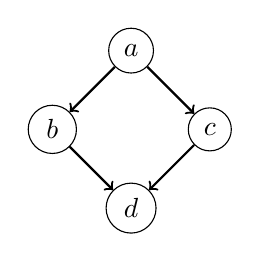
\begin{tikzpicture}
\node[draw, circle] (a) at (0,1) {$a$};
\node[draw, circle] (b) at (-1,0) {$b$};
\node[draw, circle] (c) at (1,0) {$c$};
\node[draw, circle] (d) at (0,-1) {$d$};

\draw [->, thick] (a) -- (b);
\draw [->, thick] (a) -- (c);
\draw [->, thick] (c) -- (d);
\draw [->, thick] (b) -- (d);

\end{tikzpicture}
\caption{A demonstration of the diamond problem which can give non-unique solutions to naive topological sorts on directed acyclic graphs.}\label{fig:rank_tikz_dag}
\end{figure}

To circumvent this challenge, a simple heuristic is imposed on the sorting. In cases where two nodes are interchangeable, the node with the highest outgoing edge weight sum is placed first. This draws from our context of the problem and place nodes with a greater net influence higher in such circumstances.

\subsection{Kendall rank correlation coefficient}

In order to quantify a notion of rank stability, we can run sensitivity tests on a ranking system. We do this using a simple ranking experiment. We take our network and rank it using a chosen system. We then remove a single node from the network and rerun the ranking. 

We compare these rankings using the Kendall rank correlation coefficient, referred to as Kendall's $\tau$ throughout. Kendall's $\tau$ measures the ordinal association between the two rankings with
\begin{equation}
\tau=\frac{(\text { number of concordant pairs })-(\text { number of discordant pairs })}{\binom{n}{2}},
\end{equation}
where a pair of elements $(x,y)$ are said to be concordant if the relative ordering of those two elements in both rankings is the same. The pair are discordant if $x$ ranks \emph{higher} than $y$ in one ranking and \emph{lower} in another.
If two rankings are perfectly matched $\tau$ is 1 and $\tau$ is -1 if a ranking is compared with it's reverse. 

We run the experiment, removing each node once before putting it back, to test the rank stability of the measures introduced above. When ranking is rerun on the network with a single node removed, there can be a significant change in the ordering. While many node removals result in very little ranking change in \autoref{fig:rank_boxplots}, some nodes have a large effect with the new ranking appearing close to a random reshuffle of the ordering ($\tau$ close to 0). When we compare two rankings with $n$ and $n-1$ nodes from a removal, we ignore the removed node from the original ranking order.

\begin{figure}[!htbp]
\centering
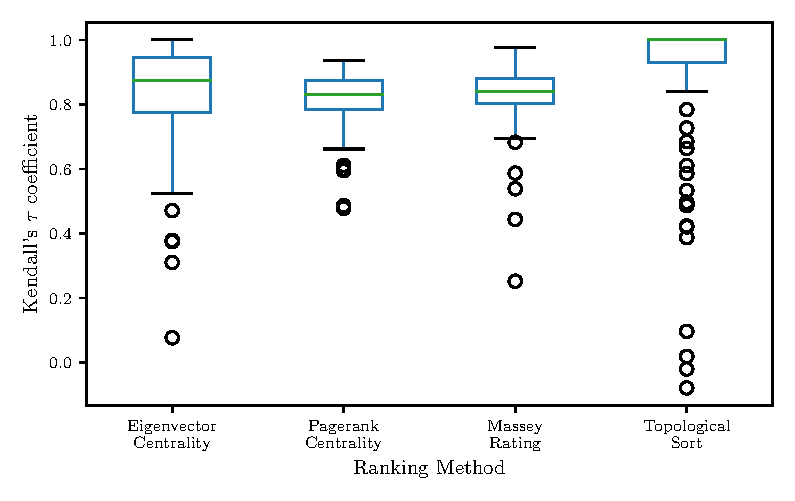
\includegraphics{chapter4/figs/removal_ranking_boxplot.pdf}
\caption{Network ranking measures undergo sensitivity testing by ranking the network with a single node removed and comparing to the original ranking. This is repeated for each possible node removal in the network for all ranking measures. All measures show an average positive correlation between new and original rankings, with a high degree of variance in the sensitivity. PageRank has the best worst-case and worse average-case while topological sorting has the best average-case and worst worst-case.}\label{fig:rank_boxplots}
\end{figure}

The eigenvector, PageRank and Massey methods all have similar characteristics of sensitivity, while the topological sorting has a slightly more skewed distribution. The directed acyclic graph means that any node removal of a leaf (a node without any children), will have no change in the ranking aside from it's removal, creating a strong cluster of results at $\tau=0$. In contrast, removal of nodes in the central paths of the DAG will likely result in a new DAG structure being generated, strongly altering the rankings.

Importantly, all of these measures have a comparable level of sensitivity, without any stand-outs. Does this mean any of the measures are sufficient as rankings? To answer this we turn to comparing the methods directly.

We use Kendall's $\tau$ to compare the ranking of the information flow network produced by each measure. Notably in \autoref{fig:rank_comparison}, all rankings have a comparative $\tau$ of less than 0.11 between each other. This score indicates that the coherence between these measures is limited. The heuristic topological sorting deviates the most from the other measures rankings, likely due to this method not using all of the non-negative adjacency matrix of the full graph.

\begin{figure}[!htbp]
\centering
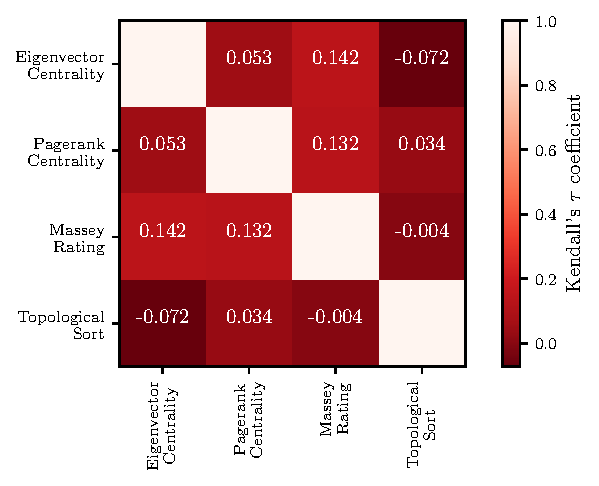
\includegraphics{chapter4/figs/compare_methods.pdf}
\caption{A comparison of the ordinal association between the rankings of each measure when applied to the information flow graph. All four measures show a limited correlation between each other, with the topological approach differing most from the non-negative matrix approaches.}\label{fig:rank_comparison}
\end{figure}

To reinforce this, \autoref{tab:ranking_top10} shows the top ten most influential news-media organisations according to each of the ranking methods. While many organisations are common to each rankings top 10, the detailed order differs significantly among each of the rankings. This is representative of the differences through the range of rankings for each method.  Full lists of rankings are available in \autoref{app:rankings_app}.


\begin{table}[!htbp]
\centering
\begin{tabular}{rlllll}
\toprule
Rank &  Eigencentraility & Pagerank &  Mossey & Topological Sort \\
\midrule
1  &        usatoday &        usatoday &   rightsidenews &       business \\
2  &        huffpost &         nytimes &        usatoday &  realdailywire \\
3  &  washingtonpost &     bostonglobe &       YahooNews &     nytopinion \\
4  &     bostonglobe &  washingtonpost &        huffpost &           time \\
5  &       YahooNews &        huffpost &       voxdotcom &      newyorker \\
6  &       voxdotcom &             npr &  washingtonpost &          NYMag \\
7  &             npr &       voxdotcom &     DeseretNews &   RollingStone \\
8  &         nytimes &     DeseretNews &     bostonglobe &    theatlantic \\
9  &     DeseretNews &         latimes &     townhallcom &    motherjones \\
10 &   rightsidenews &  WestJournalism &             npr &       rawstory \\
\bottomrule
\end{tabular}
\caption{Top 10 most influential news-media organisations according to each measure, listed as their Twitter account handles. The rankings can differ significantly across methods although many of the top 10 are shared between methods.}\label{tab:ranking_top10}
\end{table}

\section{Discussion}

% <internal consistency>
Ranking methodologies are inherently fraught with assumptions and bias. As is the case here, ranking influence in a flow graph is underpinned by a constructed notion of influence. These assumptions are contextual and can be well justified; however communicating these assumptions can be difficult when a viewer seeks a simple definitive list. This exacerbates the challenge of communication, where assumptions and bias must be so clear as to be obvious to a viewer. In some cases this is possible, such as where the ranking metric is a simple statistic (i.e.\ students average grades in a course, the market capitalisation of a company) or where the ranking principles are well established (i.e.\ the use of Elo in chess ranking). In situations where the source material is more complex -- such as the case of a flow graph -- norms and assumptions around ranking is not well established, and communication of these can prove difficult.

% <assumptions>
Even with clearly established assumptions, often no method of ranking is clearly superior. It is often dangerous to choose a single method \emph{ad-hoc}, as each method comes with it's own trade-offs. Consider the case of the Elo ranking system~\cite{elo_rating_1978}; this ranking system is only a useful comparative tool within it's own rating pool. If two individuals are ranked equally first or have the same high Elo across two sports, say chess and table tennis, it's difficult to compare how exceptional these two individuals are to each other without a knowledge of the ratings of many other players. Elo himself noted the difficulty of rating players, comparing it to ``the measurement of the position of a cork bobbing up and down on the surface of agitated water with a yard stick tied to a rope and which is swaying in the wind''~(Arpad Elo, Chess Life, 1962). Indeed, most popularly rating or ranking systems have their critics. The desire to fairly rate academic influence has brought criticism to naive citation counts in favour of alternative metrics such as the h-index~\cite{hirsch_index_2005}, which has itself spawned it's own academic niche through it's many derivatives and alternatives~\cite{alonso_h-index_2009}. 

Even in cases where methods are well respected and assumptions are well defined, these methods can have major flaws. Take for example the case of PageRank centrality discussed above. This centrality is considered robust and well established in the field of web page ranking, and underpins the original Google search engine~\cite{brin_anatomy_1998}. Despite this, PageRank centrality can have dangerous sensitivity even in the context of a web-graph~\cite{ng_link_2001}. We saw ourselves in \autoref{fig:rank_boxplots} that small changes in a complex network can have a large effect on the rankings. Many rating methods are exposed to sensitivity concerns under the right network conditions, and these risks can be hard to both account for and to communicate to a viewer.
% </assumptions>

% <meta ranking>
An alternative approach may be to join these ranking methods into a meta-ranking. These often either average various rankings or ratings, or use a voting process between methods to combine results into a final ranking. While this approach may appear a tool for `smoothing' the assumptions and bias of various methods, it can again prove treacherous as choices of methods to include and how to combine these methods can strongly alter the final rankings. The breadth of combinations of approaches cannot be understated, even when data is somewhat limited~\cite{BarrowRankingRankings2013}. While meta-ranking approaches likely do assist in creating more generally robust measures, they do not answer our fundamental problem with these rankings.
% </meta ranking>

% <purpose of ranking>
The search for a definitive ranking is a flawed venture. The purpose of information stored in a complex network is not to be over-simplified into facile representations. News is a dynamic interconnected system, which is already simplified into net information flow edges in a network. Reducing this further can lead to deeply flawed or misleading narratives, often without it being clear what error has been made. 
% </purpose of ranking>

% <what you can do>
As discussed in \autoref{sec:gowiththeflow}, the network can be used to answer some specific questions, such as in comparing magnitude difference of edges or discussing a the flow between a single pair of organisations. These question can be extended to look at local neighbourhood structure. For example, if a news-media outlet has only outgoing information flow edges, than we can definitively say that they are a completely-net-contributor of information into the ecosystem. This is true for a single node in our data, \emph{USA Today}, although these out-flowing edges are mostly low weight and therefore susceptible to error from noise.

Further, some clear network results can be extracted at the extremes of results. For example, while it may be hard to compare the total influence of the \emph{New York Times} to the total influence of the \emph{Washington Post}, we can concluded that both are more influential than \emph{Arkansas Democrat-Gazette} based on the rankings from all methods. 
% </what you can do>

% ending
While this chapter does not provide a convenient definitive ranking, it highlights the caution needed in investigating the network, as any result is grounded in the assumption made during the analysis. This difficulty in creating a clean ranking reflects in inherent complexity in the network of information flows and highlights the fact that the news ecosystem is itself complex. 

% % old ending
% This chapter opened with a question: which news organisations are the most important information sources? We answer this question not with a canonical list, but rather with a variety of tools with which one can probe this question from different angles., but should be used as guides and tools, not encompassing answers.